\subsection{Hyperparameter Tuning}
One important deviation from the guiding paper is in data normalization. Tian et.al, normalized the VGT and PH using an empirical measure of the timescale
\begin{equation}
    \tau \approx \langle \norm{S^2} \rangle^{-1}
\end{equation}
In our work, we confirmed it was vital to performance to normalize the VGT
\begin{equation}
    A' = \tau A
\end{equation}
but found the network performance suffered considerably if the PH was normalized. One hypothesis is that this is an artifact of initialization of the network parameters. The PH should be normalized by $\tau^2$, which for $Re=240$ $\tau \approx 3e-3$. If one uses this normalization, the network does train, but it seems to start very far away from the optimal. It is possible this could remedied by scaling the initialization of the linear output layer as well as individualizing that layer's learning rate - this was not performed.

In calculation of the $g^{(i)}$ functions, we use a fully connected feed-forward network with 5 hidden layers of 50 nodes apiece with relu activation functions and a linear output layer. This network is trained using the ADAM optimizer with learning rate $5e-3$ decaying to a minimum of $1e-6$ via factors of $2$ when the loss reaches a plateau. 

\subsection{Result reproduction}
After implementing this network architecture and finding the hyperparameters above, the results in figure(\ref{fig:tbnn_reproduction_results}) were found. These results agree well with the original paper, and suggest the hyperparameter choices were accurate.

\begin{figure}
    \centering
    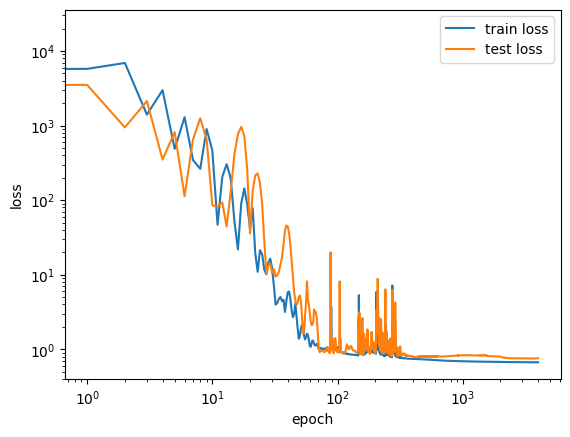
\includegraphics[width=0.5\textwidth]{LagrangianDeformationModels/figs/trained_tbnn_loss.png}%
    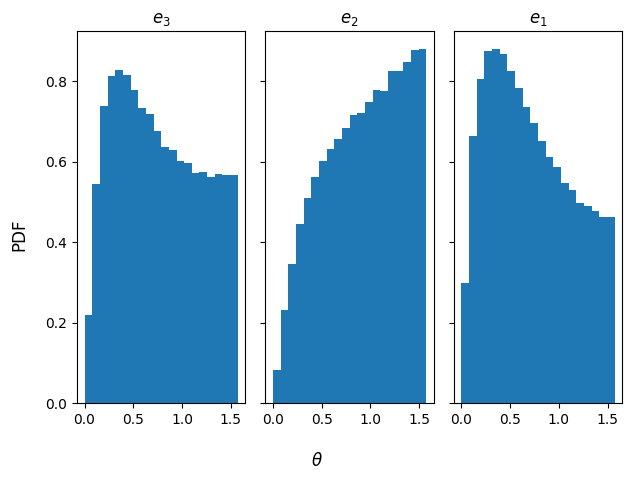
\includegraphics[width=0.5\textwidth]{LagrangianDeformationModels/figs/tbnn_ph_eig_align.png}
    \caption{(left) Loss as a function of epoch for the TBNN, (right) PDFs of eigenvalue alignment for the pressure hessian, sorted from smallest to largest eigenvalue left to right. These plots agree well with results from Tian et.al's paper, suggesting the implementation is correct.}
    \label{fig:tbnn_reproduction_results}
\end{figure}

\begin{figure}
    \centering
    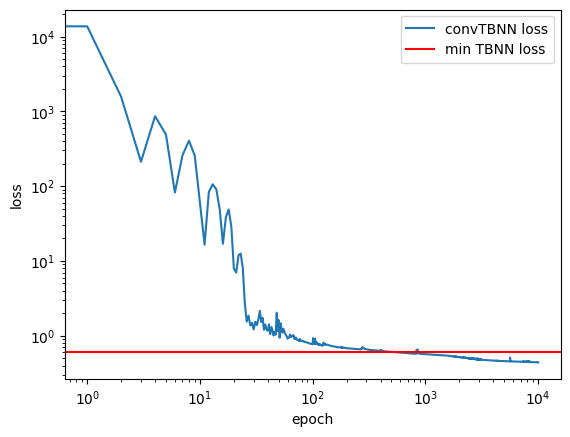
\includegraphics[width=0.5\textwidth]{LagrangianDeformationModels/figs/conv_tbnn_loss.png}%
    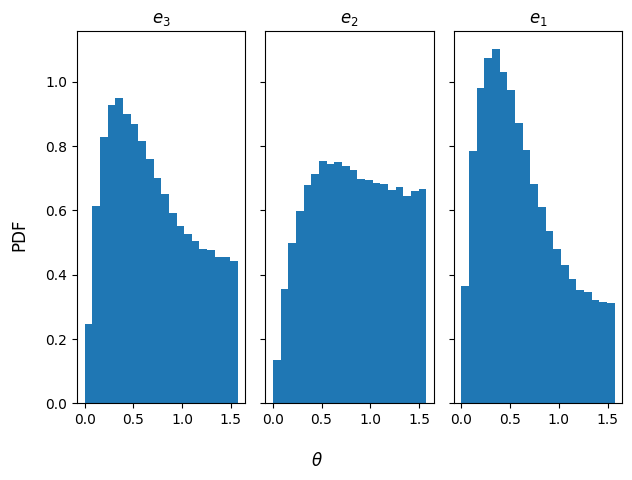
\includegraphics[width=0.5\textwidth]{LagrangianDeformationModels/figs/conv_tbnn_ph_eig_align.png}
    \caption{Preliminary results of training the convTBNN. (Left) shows the loss vs epoch, with the minimum loss obtained by the unmodified TBNN marked in horizontal red, and the convTBNN in blue. (Right) shows the alignment PDFs of eigenvectors of the PH. Here $e_1$ corresponds to the eigenvector with the greatest associated eigenvalue. Note that compared to fig(\ref{fig:tbnn_reproduction_results}), all alignment PDFs are better, shifting significant density from the misaligned (larger $\theta$) to aligned.}
    \label{fig:conv_tbnn_results}
\end{figure}

\subsection{Temporal Convolution TBNN}
Preliminary results suggest that the additional historical information of the VGT is in fact useful for the prediction of the PH. In figure(\ref{fig:conv_tbnn_results}), results of training the temporal convolution TBNN (convTBNN) are shown, improving both in the loss and eigenvector alignment metrics.

\begin{figure}
    \centering
    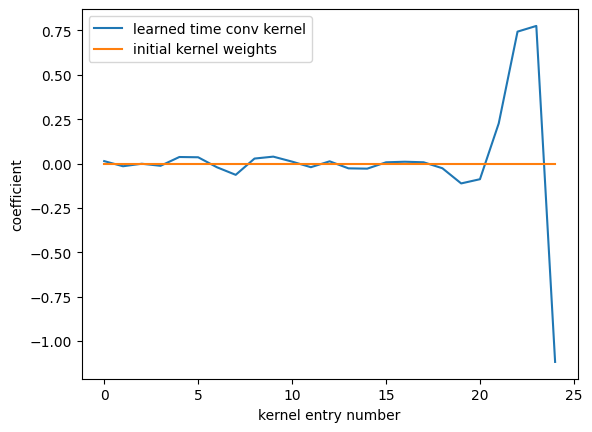
\includegraphics[width=0.5\textwidth]{LagrangianDeformationModels/figs/temporal_conv_kernel.png}
    \caption{The weights of the learned temporal convolution kernel. This may act as a stand-in for a measure of significance for VGT history as it relates to the prediction of the PH. If these results hold across many trainings, it would suggest that only "recent" history is informative in prediction of the PH.}
    \label{fig:conv_kernel}
\end{figure}
An interesting aspect of the convTBNN is the ability to inspect the kernel length - loosely the length over which the network found it useful to set weights away from zero. Figure(\ref{fig:conv_kernel}) displays the weights as a function of kernel entry number. The sampling in time occurs every $20\Delta t$, where $\Delta t = 3e-4$ and the Kolmogorov timescale is $\tau \approx 3e-3$, so that the sampling occurs about every $2\tau$. We see that only the last three weights are nonzero, suggesting that a history of about $6\tau$ is useful in prediction.